\documentclass[onecolumn]{IEEEtran}
\usepackage[brazilian]{babel}
\usepackage[utf8]{inputenc}
\usepackage[T1]{fontenc}

\usepackage{ amssymb }

% \usepackage{epstopdf}
\usepackage{graphicx}

\usepackage{lipsum}


\title{Teoria da Informação - Homework 05}
\author{Yuri Niitsuma}
\date{October 2017}

\begin{document}
\maketitle

\begin{enumerate}
\itemsep1em

    \section*{Exercises.}
	
	\item
	The following exercises regard stream codes.
	\begin{enumerate}
	    \item
	    (MacKay 6.5) [Medium]
Encode the string $000000000000100000000000$ using the basic Lempel-Ziv algorithm described above.

\subsection*{Resposta}

\includegraphics[width=0.5\textwidth]{img/01.pdf}
    	\item
    	(MacKay 6.6) [Medium]

Decode the string

\[00101011101100100100011010101000011\]

that was encoded using the basic Lempel-Ziv algorithm.

\subsection*{Resposta}

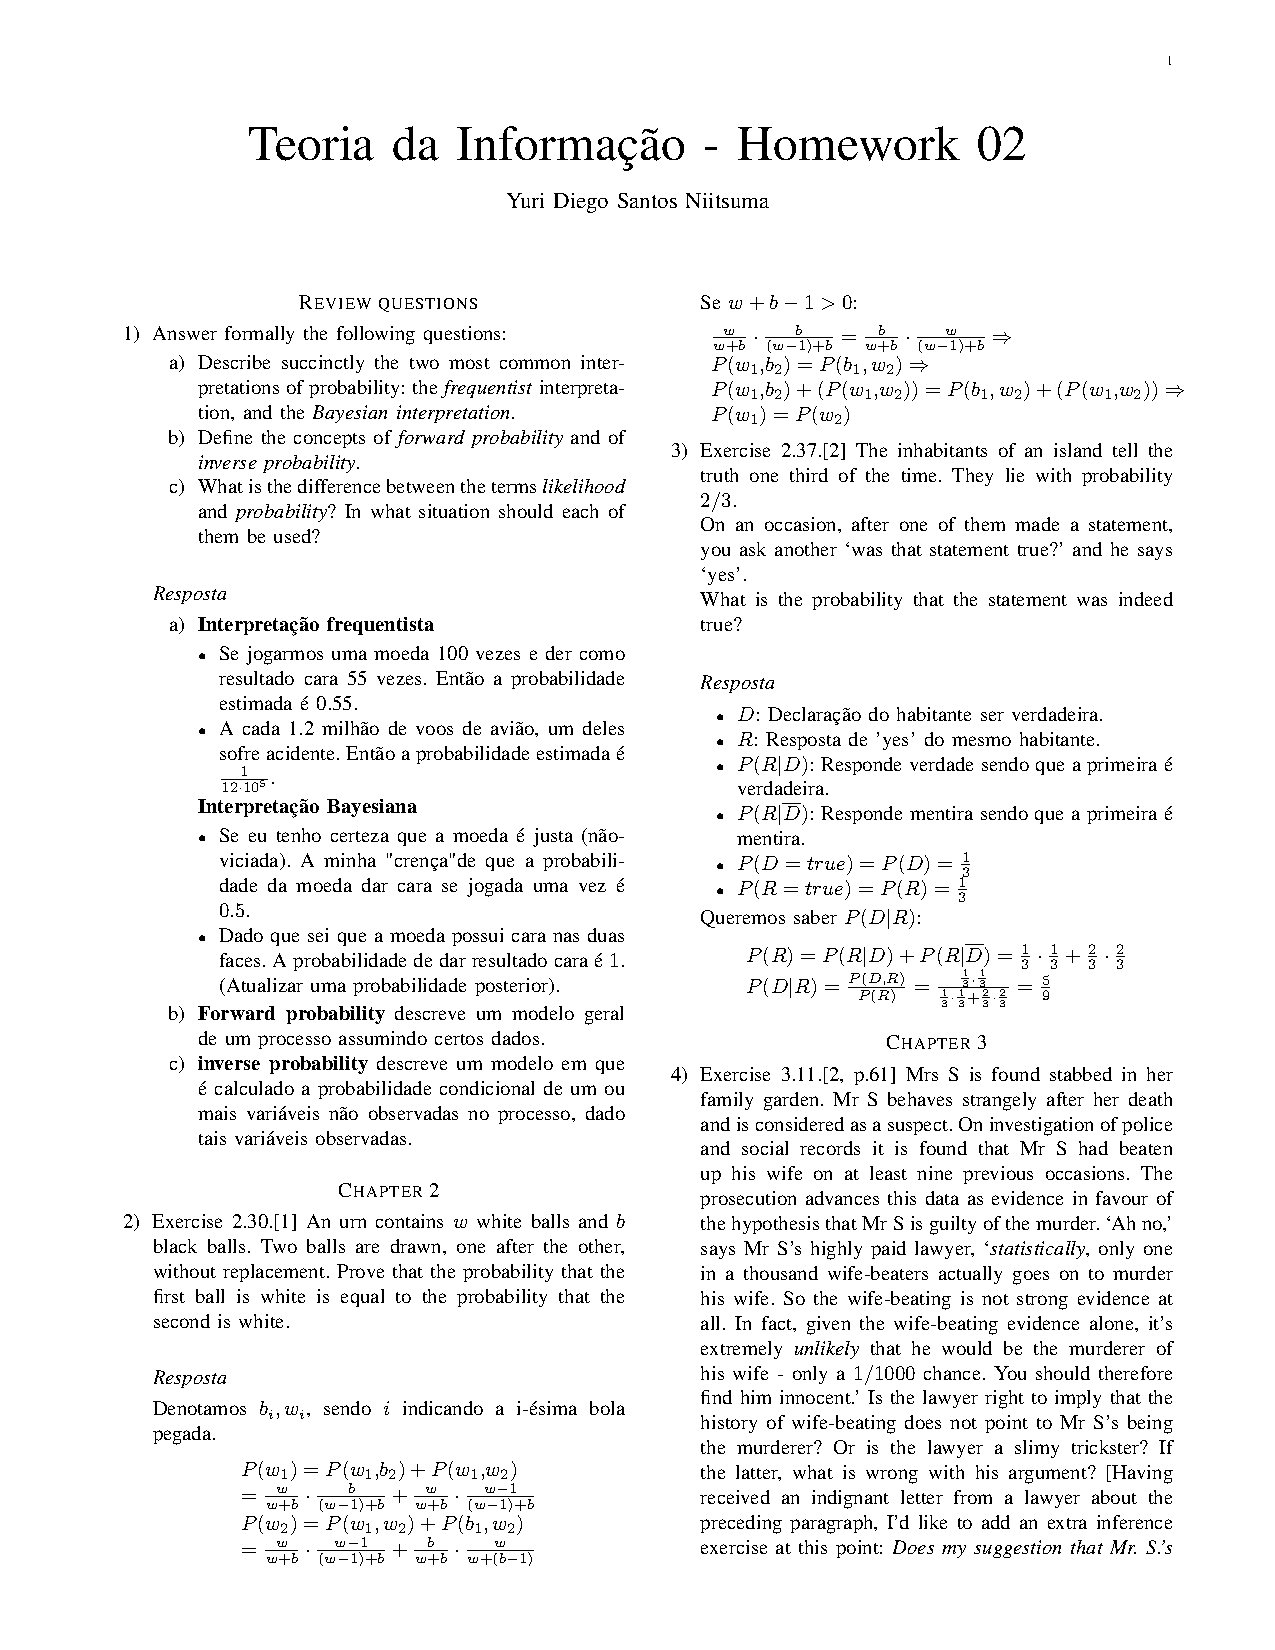
\includegraphics[width=0.5\textwidth]{img/02.pdf}

	\end{enumerate}
    \bigskip
    
    \newpage
    \item
        \textbf{(The entropy of a compressed file)} This exercise regards compression algorithms in general.

An information theory student wants to check whether she can beat Shannon's compression limit of $H(X)$ bits per symbol for an optimal code $C$ applied to a source $X$.

She envisions a lossless compression method in two steps as follows:

\textbf{Step 1:} Apply an optimal lossless code $C$ to the source $X$, obtaining a compressed file $Y$.

\textbf{Step 2:} Apply a new optimal lossless code $C'$ to the source $Y$, obtaining a new compressed file $Z$.

Recalling Shannon's Source Coding Theorem, the student makes the following claims about her newly proposed compressing method:

\textbf{Claim 1:} Since code $C$ is optimal for the source $X$, file $Y$ uses approximately $H(X)$ bits to represent each symbol of $X$.

\textbf{Claim 2:} Since code $C'$ is optimal for the source $Y$, file $Z$ uses approximately $H(Y)$ bits to represent each symbol of $Y$.

\textbf{Claim 3:} File $Z$ represents each symbol of $X$ using approximately $H(X)H(Y)$ bits.

\begin{enumerate}
	\item
	${\rm{[Easy]}}$ Discuss whether or not each of the student's three claims are correct.

	\item
	${\rm{[Medium]}}$ What can we say about the size of file $Y$ in comparison to the size of file $Z$? Is $Z$ gonna be smaller, larger, or of equal size to $Y$? (Hint: Recall that Shannon's Source Coding Theorem must be valid for the compression from $X$ to $Z$.)

	\item
	${\rm{[Medium]}}$ Using your answers to the previous items, what would be an accurate estimation for the value of $H(Y)$?

	\item
	${\rm{[Medium]}}$ Using your answers to the previous items, what can the student conclude about the frequency of bits $0$ and $1$ in any optimally compressed file? How does that relate to the title of this assignment: "\textit{Compression and redundancy}"?
	
\end{enumerate}

\subsection*{Resposta}

\begin{enumerate}
\itemsep1em

    \item 
    \textit{Claims} 1 e 2 são colorários do Teorema de Codificação da Fonte. \\
    Para provar o 3: \\
    \begin{itemize}
        \item Cada símbolo de $X$ é representado em $Y$ utilizando $H(X)$ bits.
        \item Cada símbolo de $Y$ é representado em $Z$ utilizando $H(Y)$ bits.
        \item Cada símbolo de $X$ é representado em $Z$ utilizando $H(X)H(Y)$ bits.
    \end{itemize}
    
    % Claims 1 and 2 are direct consequences of Shannon's Source Coding Theorem.
    % Claim 3 follows immediately from the previous two claims: since each symbol of X is represented in Y using H(X) bits, and each symbol of Y (note that each symbol of Y is itself a bit) is represented in Z using H(Y ) bits, we have that each symbol of X is represented using H(X)H(Y ) bits in Z.
    
    \item
    O Teorema de Codificação da Fonte diz que tem que valer a compressão de $X$ pra $Z$, não importando se o roda em uma, duas ou qualquer quantidade de vezes. Desde, $Z$ não pode ser menor que $Y$, por outro lado podemos ter uma compressão que bate o limite de Shannon um arquivo utilizando menos que o uso de bits esperado para $X$ por símbolo da fonte. Logo, o tamanho de $Z$ tem que ser aproximadamente o mesmo tamanho de $Y$.
    % Shannon's Source Coding Theorem must be valid for the compression from X to Z, no matter whether the algorithm runs in one, two, or whatever number of steps. Hence, Z cannot be smaller than Y , otherwise we would have a compression that beats Shannon limit by producing an output file using less than H(X) bits per symbol of the source file. That means that the size of Z must be approximately the same size of Y .
    
    \item 
    Do \textit{claim} 3, $Z$ utiliza $H(X)H(Y)$ bits por símbolo de $X$ e $H(X)$ por símbolo de $X$. Logo, temos que $H(Y)$ é muito próximo de $1$ bit.
    % From Claim 3 we know that Z uses H(X)H(Y ) bits per symbol of X, and from (1b) we know that Z uses H(X) bits per symbol of X. Hence, we must conclude that $H(Y) \approx 1$.
    
    \item 
    $H(Y) \approx 1$ implica que os bits $0$ e $1$ ocorrem com aproximadamente com mesma frequência em $Y$. A compressão ótima remove toda redundância da fonte produzindo uma compressão em que a frequência de $0$'s e $1$'s é uniforme.
    % From (1c) we know that $H(Y) \approx 1$, which means that bits 0 and 1 must occur approximately with equal frequency in Y . This is a general charecteristic of optimal compressors: they remove all redundancy from the source file, producing a compressed file in which the frequency of 0's and 1's is uniform.

\end{enumerate}

\end{enumerate}

\end{document}
